\documentclass[reqno, 12pt]{amsart}
\usepackage{amsmath,graphicx}
\usepackage{amssymb,amsthm}
\usepackage{xcolor}
\usepackage[T1]{fontenc}
\usepackage{tikz}
\usetikzlibrary{calc,decorations.pathmorphing}
\pgfdeclarelayer{background}
\pgfdeclarelayer{foreground}
\pgfdeclarelayer{front}
\pgfsetlayers{background,main,foreground,front}

\begin{document}

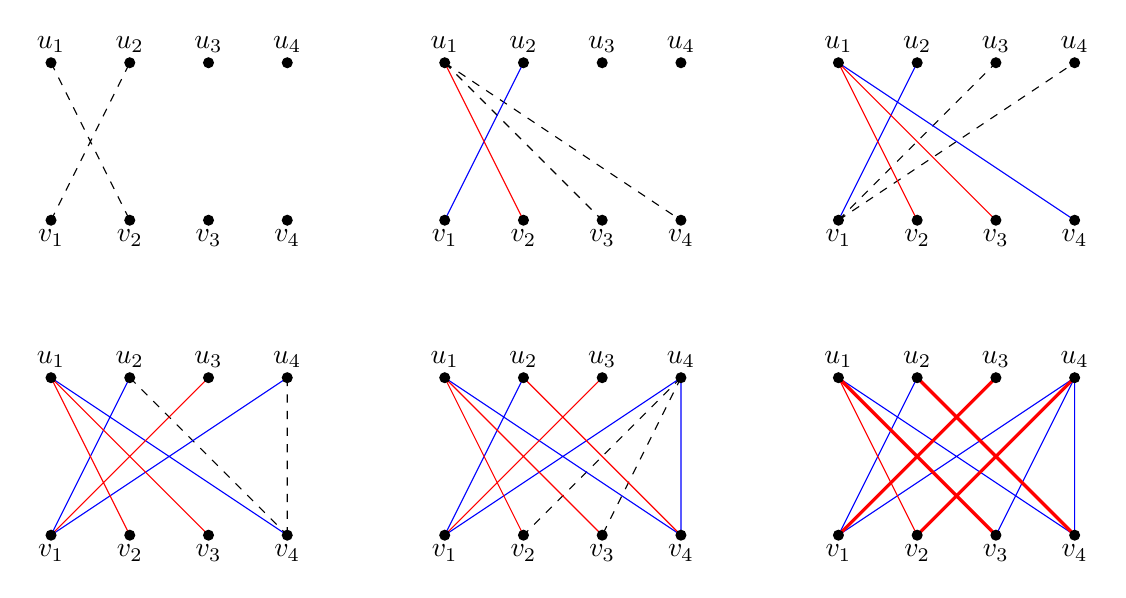
\begin{tikzpicture}
    \centering
    \coordinate (u1) at (0,1);
    \coordinate (u2) at (1,1);
    \coordinate (u3) at (2,1);
    \coordinate (u4) at (3,1);
    \coordinate (v1) at (0,-1);
    \coordinate (v2) at (1,-1);
    \coordinate (v3) at (2,-1);
    \coordinate (v4) at (3,-1);
    \begin{pgfonlayer}{front}
        \draw[dashed] (v1) -- (u2) (u1) -- (v2); 
        \foreach \i in {v1,v2,v3,v4,u1,u2,u3,u4} \fill (\i) circle (2pt);	
        \node at (0,1) [above] {$u_1$};
        \node at (1,1) [above] {$u_2$};
        \node at (2,1) [above] {$u_3$};
        \node at (3,1) [above] {$u_4$};
        \node at (0,-1) [below] {$v_1$};
        \node at (1,-1) [below] {$v_2$};
        \node at (2,-1) [below] {$v_3$};
        \node at (3,-1) [below] {$v_4$};
    \end{pgfonlayer}

    \coordinate (u1) at (5,1);
    \coordinate (u2) at (6,1);
    \coordinate (u3) at (7,1);
    \coordinate (u4) at (8,1);
    \coordinate (v1) at (5,-1);
    \coordinate (v2) at (6,-1);
    \coordinate (v3) at (7,-1);
    \coordinate (v4) at (8,-1);
    \begin{pgfonlayer}{front}
        \draw[dashed] (u1) -- (v3) (u1) -- (v4);
        \draw[blue] (v1) -- (u2);
        \draw[red] (u1) -- (v2); 
        \foreach \i in {v1,v2,v3,v4,u1,u2,u3,u4} \fill (\i) circle (2pt);	
        \node at (5,1) [above] {$u_1$};
        \node at (6,1) [above] {$u_2$};
        \node at (7,1) [above] {$u_3$};
        \node at (8,1) [above] {$u_4$};
        \node at (5,-1) [below] {$v_1$};
        \node at (6,-1) [below] {$v_2$};
        \node at (7,-1) [below] {$v_3$};
        \node at (8,-1) [below] {$v_4$};
    \end{pgfonlayer}

    \coordinate (u1) at (10,1);
    \coordinate (u2) at (11,1);
    \coordinate (u3) at (12,1);
    \coordinate (u4) at (13,1);
    \coordinate (v1) at (10,-1);
    \coordinate (v2) at (11,-1);
    \coordinate (v3) at (12,-1);
    \coordinate (v4) at (13,-1);
    \begin{pgfonlayer}{front}
        \draw[dashed] (v1) -- (u3) (v1) -- (u4);
        \draw[blue] (v1) -- (u2) (u1) -- (v4);
        \draw[red] (u1) -- (v2) (u1) -- (v3); 
        \foreach \i in {v1,v2,v3,v4,u1,u2,u3,u4} \fill (\i) circle (2pt);	
        \node at (10,1) [above] {$u_1$};
        \node at (11,1) [above] {$u_2$};
        \node at (12,1) [above] {$u_3$};
        \node at (13,1) [above] {$u_4$};
        \node at (10,-1) [below] {$v_1$};
        \node at (11,-1) [below] {$v_2$};
        \node at (12,-1) [below] {$v_3$};
        \node at (13,-1) [below] {$v_4$};
    \end{pgfonlayer}

    \coordinate (u1) at (0,-3);
    \coordinate (u2) at (1,-3);
    \coordinate (u3) at (2,-3);
    \coordinate (u4) at (3,-3);
    \coordinate (v1) at (0,-5);
    \coordinate (v2) at (1,-5);
    \coordinate (v3) at (2,-5);
    \coordinate (v4) at (3,-5);
    \begin{pgfonlayer}{front}	
        \draw[dashed] (u2) -- (v4) (u4) -- (v4);
        \draw[blue] (v1) -- (u2) (u1) -- (v4) (v1) -- (u4);
        \draw[red] (u1) -- (v2) (u1) -- (v3) (v1) -- (u3); 
        \foreach \i in {v1,v2,v3,v4,u1,u2,u3,u4} \fill (\i) circle (2pt);
        \node at (0,-3) [above] {$u_1$};
        \node at (1,-3) [above] {$u_2$};
        \node at (2,-3) [above] {$u_3$};
        \node at (3,-3) [above] {$u_4$};
        \node at (0,-5) [below] {$v_1$};
        \node at (1,-5) [below] {$v_2$};
        \node at (2,-5) [below] {$v_3$};
        \node at (3,-5) [below] {$v_4$};
    \end{pgfonlayer}

    \coordinate (u1) at (5,-3);
    \coordinate (u2) at (6,-3);
    \coordinate (u3) at (7,-3);
    \coordinate (u4) at (8,-3);
    \coordinate (v1) at (5,-5);
    \coordinate (v2) at (6,-5);
    \coordinate (v3) at (7,-5);
    \coordinate (v4) at (8,-5);
    \begin{pgfonlayer}{front}
        \draw[dashed] (u4) -- (v2) (u4) -- (v3);
        \draw[blue] (v1) -- (u2) (u1) -- (v4) (v1) -- (u4) (u4) -- (v4);
        \draw[red] (u1) -- (v2) (u1) -- (v3) (v1) -- (u3) (u2) -- (v4);
        \foreach \i in {v1,v2,v3,v4,u1,u2,u3,u4} \fill (\i) circle (2pt);
        \node at (5,-3) [above] {$u_1$};
        \node at (6,-3) [above] {$u_2$};
        \node at (7,-3) [above] {$u_3$};
        \node at (8,-3) [above] {$u_4$};
        \node at (5,-5) [below] {$v_1$};
        \node at (6,-5) [below] {$v_2$};
        \node at (7,-5) [below] {$v_3$};
        \node at (8,-5) [below] {$v_4$};
    \end{pgfonlayer}

    \coordinate (u1) at (10,-3);
    \coordinate (u2) at (11,-3);
    \coordinate (u3) at (12,-3);
    \coordinate (u4) at (13,-3);
    \coordinate (v1) at (10,-5);
    \coordinate (v2) at (11,-5);
    \coordinate (v3) at (12,-5);
    \coordinate (v4) at (13,-5);
    \begin{pgfonlayer}{front}
        \draw[blue] (v1) -- (u2) (u1) -- (v4) (v1) -- (u4) (u4) -- (v4) (u4) -- (v3);
        \draw[red] (u1) -- (v2);
        \draw[red, very thick] (u1) -- (v3) (v1) -- (u3) (u2) -- (v4) (u4) -- (v2);
        \foreach \i in {v1,v2,v3,v4,u1,u2,u3,u4} \fill (\i) circle (2pt);	
        \node at (10,-3) [above] {$u_1$};
        \node at (11,-3) [above] {$u_2$};
        \node at (12,-3) [above] {$u_3$};
        \node at (13,-3) [above] {$u_4$};
        \node at (10,-5) [below] {$v_1$};
        \node at (11,-5) [below] {$v_2$};
        \node at (12,-5) [below] {$v_3$};
        \node at (13,-5) [below] {$v_4$};
    \end{pgfonlayer}
\end{tikzpicture}

\end{document}